%----------------------------------------------------------------------------------------
%	PACKAGES AND THEMES
%----------------------------------------------------------------------------------------

\documentclass{beamer}

\mode<presentation> {

% The Beamer class comes with a number of default slide themes
% which change the colors and layouts of slides. Below this is a list
% of all the themes, uncomment each in turn to see what they look like.

%\usetheme{default}
%\usetheme{AnnArbor}
%\usetheme{Antibes}
%\usetheme{Bergen}
%\usetheme{Berkeley}
%\usetheme{Berlin}
%\usetheme{Boadilla}
%\usetheme{CambridgeUS}
%\usetheme{Copenhagen}
%\usetheme{Darmstadt}
%\usetheme{Dresden}
%\usetheme{Frankfurt}
%\usetheme{Goettingen}
%\usetheme{Hannover}
%\usetheme{Ilmenau}
%\usetheme{JuanLesPins}
%\usetheme{Luebeck}
%\usetheme{Madrid}
%\usetheme{Malmoe}
%\usetheme{Marburg}
%\usetheme{Montpellier}
%\usetheme{PaloAlto}
\usetheme{Pittsburgh}
%\usetheme{Rochester}
%\usetheme{Singapore}
%\usetheme{Szeged}
%\usetheme{Warsaw}

% As well as themes, the Beamer class has a number of color themes
% for any slide theme. Uncomment each of these in turn to see how it
% changes the colors of your current slide theme.

%\usecolortheme{albatross}
%\usecolortheme{beaver}
%\usecolortheme{beetle}
%\usecolortheme{crane}
%\usecolortheme{dolphin}
%\usecolortheme{dove}
%\usecolortheme{fly}
%\usecolortheme{lily}
%\usecolortheme{orchid}
%\usecolortheme{rose}
%\usecolortheme{seagull}
%\usecolortheme{seahorse}
%\usecolortheme{whale}
%\usecolortheme{wolverine}

%\setbeamertemplate{footline} % To remove the footer line in all slides uncomment this line
%\setbeamertemplate{footline}[page number] % To replace the footer line in all slides with a simple slide count uncomment this line

%\setbeamertemplate{navigation symbols}{} % To remove the navigation symbols from the bottom of all slides uncomment this line
}

\usepackage{graphicx} % Allows including images
\usepackage{booktabs} % Allows the use of \toprule, \midrule and \bottomrule in tables

\usepackage[english,russian]{babel}
\usepackage[utf8x]{inputenc}
\selectlanguage{russian}
\usepackage{amssymb}
%----------------------------------------------------------------------------------------
%	TITLE PAGE
%----------------------------------------------------------------------------------------

\title[Граф дорог]{Кратчайшие пути в графе дорог} % The short title appears at the bottom of every slide, the full title is only on the title page

\author{Андроник Ордиян\\ \textbf{Научный руководитель}: Алексей Гуревич} % Your name
\institute[SPbAU] % Your institution as it will appear on the bottom of every slide, may be shorthand to save space
{

Академический университет  \\% Your institution for the title page

%\textit{andronik.ordian@gmail.com} % Your email address
}
\date{\today} % Date, can be changed to a custom date

\begin{document}

\begin{frame}
\titlepage % Print the title page as the first slide
\end{frame}

\begin{frame}
\frametitle{Обзор} % Table of contents slide, comment this block out to remove it
\tableofcontents % Throughout your presentation, if you choose to use \section{} and \subsection{} commands, these will automatically be printed on this slide as an overview of your presentation
\end{frame}

%----------------------------------------------------------------------------------------
%	PRESENTATION SLIDES
%----------------------------------------------------------------------------------------

%------------------------------------------------
\section{Введение} % Sections can be created in order to organize your presentation into discrete blocks, all sections and subsections are automatically printed in the table of contents as an overview of the talk
%------------------------------------------------

\begin{frame}
\frametitle{Задача кратчайшего пути}
\begin{columns}[c] % The "c" option specifies centered vertical alignment while the "t" option is used for top vertical alignment

\column{.45\textwidth} % Left column and width
\textbf{Вход}
\begin{itemize}
\item Орграф $G = (V, E)$
\item Веса рёбер $w(u, v) \geq 0$
\item Начальная вершина $s$
\item Конечная вершина $t$
\end{itemize}

\textbf{Цель: найти кратчайший путь от $s$ до $t$}
\begin{itemize}
\item $V$ -- перекрёстки $\sim 10^7$
\item $E$ -- отрезки дорог, их соединяющие $\sim 10^7$
\item $w(u,v)$ -- расстояние или время в пути
\end{itemize}

\column{.5\textwidth} % Right column and width
\includegraphics[scale=0.2]{yandex.jpg}

\end{columns}
\end{frame}

%------------------------------------------------

%------------------------------------------------
\section{Мотивация}
%------------------------------------------------

\begin{frame}
\frametitle{Мотивация}
\begin{enumerate}

\item Используется в:

  \begin{itemize}
  \item Яндекс.Карты, Google.Maps, Yahoo! Maps
  \item Mapquest, Microsoft MapPoint
  \item GPS устройства
  \item Приближение для задачи TSP
  \item Некоторые задачи AI
  \item и т.д.
  \end{itemize}

\item Не всё так просто:

  \begin{itemize}
  \item Алгоритм Дейкстры не слишком быстрый
  \item Предпосчитать всё заранее не получится:
  	\begin{itemize}	
    \item время (Европа): $n \times Dijkstra \sim 5$ лет 
    \item память(Европа): $n \times n$ таблица $\sim 1$ петабайт  
    \end{itemize}
  \item Нужно нечто среднее
  \end{itemize}
  
\end{enumerate}

\end{frame}

%------------------------------------------------

%------------------------------------------------
\section{Алгоритмы}
%------------------------------------------------

%------------------------------------------------

\begin{frame}
\frametitle{Двунаправленный алгоритм}
\begin{block}{Двунаправленный Дейкстра}
  \begin{itemize}	
  \item запускаем \textbf{forward} Dijkstra от $s$, находим $d_f(v)$ 
  \item запускаем \textbf{reverse} Dijkstra от $t$, находим $d_r(v)$
  \item переключаемся после каждой итерации
  \end{itemize}
\end{block}

\begin{block}{Когда найдётся вершина просканированная дважды:}
  \begin{itemize}	
  \item просматриваем все рёбра с концами, просмотренными разными Dijkstra
  \item находим минимум $d_f(u) + w(u, v) + d_r(v)$
  \end{itemize}
\end{block}
\end{frame}

%------------------------------------------------

\begin{frame}
\frametitle{Алгоритм Дейкстры}
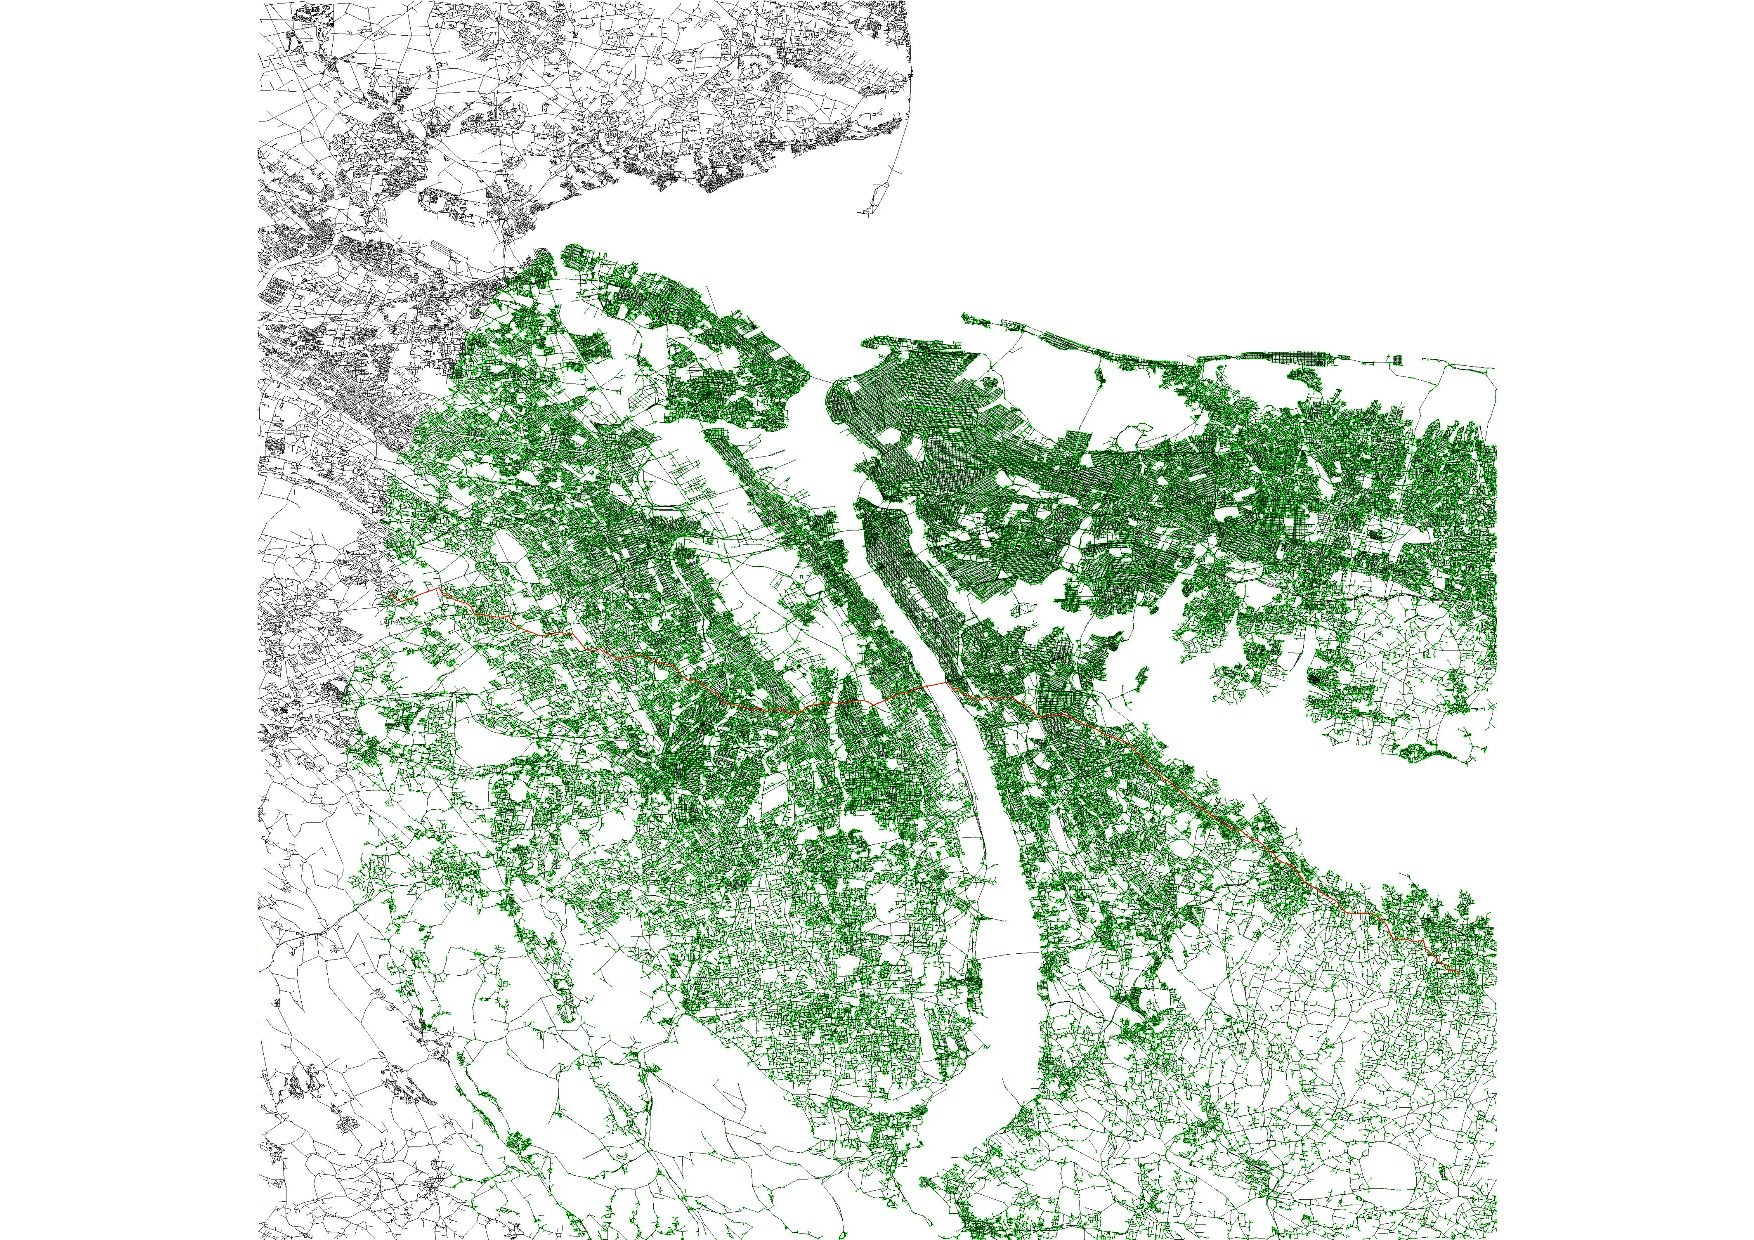
\includegraphics[width=\textwidth, page={1}]{dijkstra_12_100000.pdf}
\end{frame}

%------------------------------------------------

\begin{frame}
\frametitle{Двунаправленный Дейкстра}
\includegraphics[width=\textwidth, page={2}]{dijkstra_12_100000.pdf}
\end{frame}

%------------------------------------------------

\begin{frame}
\frametitle{Сравнение}
\begin{table}
\begin{tabular}{l l l l l}
\toprule
\textbf{Метод} & \textbf{Предподсчёт (сек./mb)} & \textbf{scaned} 
& \textbf{ms}\\
\midrule
Dijkstra    & ---/30 & 506708 & 416.569\\
biDijkstra  & ---/30 & 380603 & 361.195\\
\bottomrule
\end{tabular}
\caption{США, Флорида, 1.2 млн}
\end{table}
\end{frame}

%------------------------------------------------

\begin{frame}
\frametitle{A* поиск}
\begin{itemize}	
  \item Возьмём любую функцию (потенциала) $\pi \colon V \to \mathbb{R}$
  \item A* поиск $\equiv$ Dijkstra с расстоянием $w_\pi$
  \item $w_{\pi}(u,v) = w(u, v) - \pi(u) + \pi(v)$
  \item Для корректности нужно: $w_{\pi} \geq 0$
  \item $\pi$ даёт нижнуюю оценку на расстояние
  \item Чем точнее оценка, тем быстрее сходимость
  \item Эффект: \textbf{целенаправленный} поиск
\end{itemize}
\end{frame}

%------------------------------------------------

\begin{frame}
\frametitle{Двунаправленный A* поиск}
\begin{enumerate}

\item Нужно две функции потенциала: $\pi_f$ и $\pi_r$
\item Проблема: получатся разные расстояния!
\item Решение: усредняем потенциалы 
\item $\pi_f = \frac{\pi_f - \pi_r}{2}$
\item $\pi_r = \frac{\pi_r - \pi_f}{2}$
\end{enumerate}

\end{frame}

%------------------------------------------------

\begin{frame}
\frametitle{A* поиск}
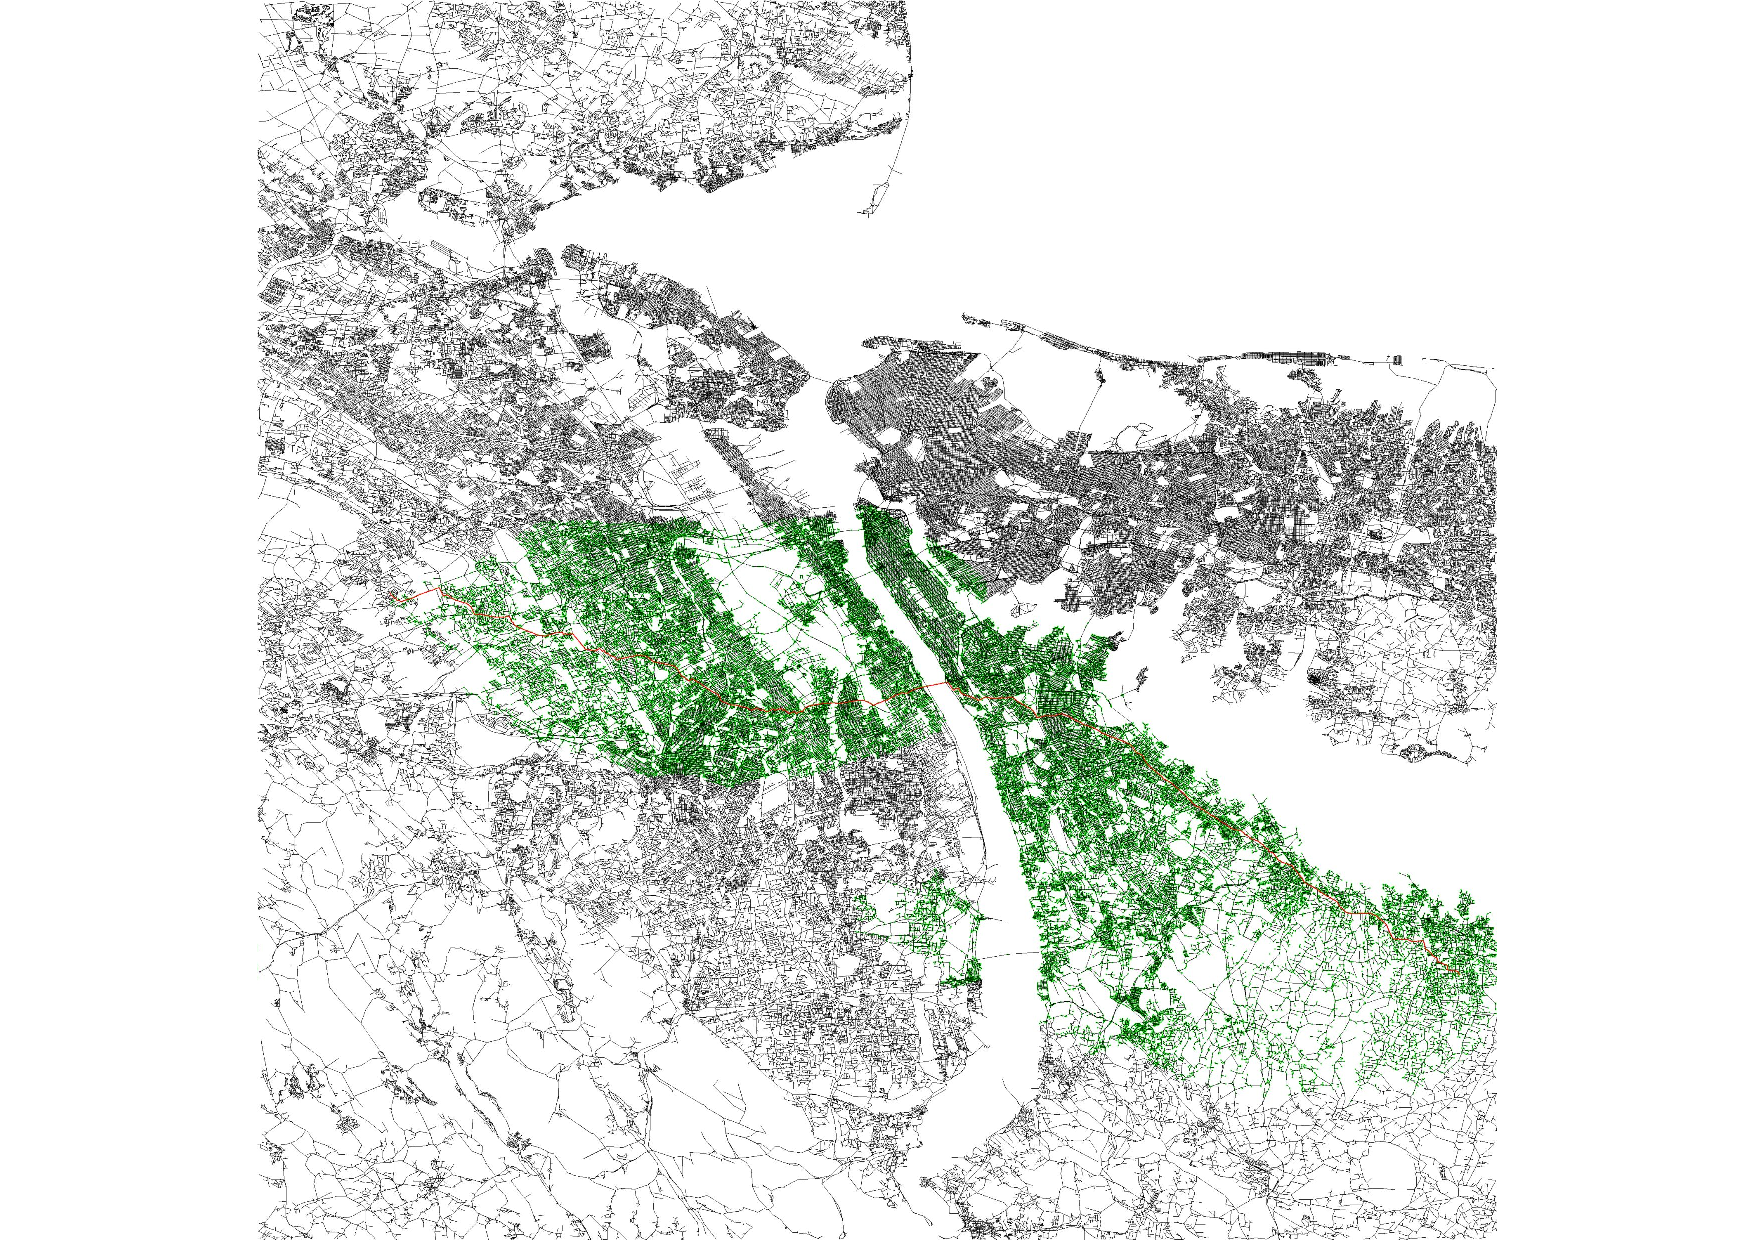
\includegraphics[width=\textwidth, page={1}]{aStar_12_100000.pdf}
\end{frame}

%------------------------------------------------

\begin{frame}
\frametitle{Двунаправленный A*}
\includegraphics[width=\textwidth, page={2}]{aStar_12_100000.pdf}
\end{frame}

%------------------------------------------------

\begin{frame}
\frametitle{Сравнение}
\begin{table}
\begin{tabular}{l l l l l}
\toprule
\textbf{Метод} & \textbf{Предподсчёт (сек./mb)} & \textbf{scaned} 
& \textbf{ms}\\
\midrule
Dijkstra    & ---/30 & 506708 & 416.569\\
biDijkstra  & ---/30 & 380603 & 361.195\\
A*          & ---/30 & 161969 & 206.392\\
biA*        & ---/30 & 149847 & 222.381\\
\bottomrule
\end{tabular}
\caption{США, Флорида, 1.2 млн}
\end{table}
\end{frame}

%------------------------------------------------

\begin{frame}
\frametitle{ALT}
\begin{itemize}	
  \item \textbf{A}* + \textbf{L}andmarks + 	\textbf{T}riangle inequality: \textbf{ALT} \cite{p1} 
  \item Предподсчёт: выбираем несколько (например, 16) вершин как \textbf{ориентиры}
  \item Считаем расстояние от них до всех остальных
  \item Сохраняем эти расстояния
  \item Запрос: A* поиск с ориентирами, используя неравенство треугольника
\end{itemize}
\end{frame}

%------------------------------------------------


\begin{frame}
\frametitle{ALT}
\begin{enumerate}	
\item Используем неравенство $\triangle$
	$$dist(u, v) \geq dist(A, v) - dist(A, u)$$
    $$dist(u, v) \geq dist(u, A) - dist(v, A)$$
\item Выбираем максимум нижних границ по всем ориентирам
\item Больше ориентиров $\Rightarrow$ точнее оценка, больше памяти
\end{enumerate}
\end{frame}

%------------------------------------------------

\begin{frame}
\frametitle{ALT: выбор ориентиров}
\begin{enumerate}	
\item Нужно выбрать ориентиры, которые хороши для всех запросов
\item Несколько видов было опробовано:
	\begin{itemize}
    \item random
    \item planar
    \item avoid
    \end{itemize}
\end{enumerate}
\end{frame}

%------------------------------------------------

\begin{frame}
\frametitle{ALT: planar ориентиры}
\begin{enumerate}	
\item Делим карту на $n$ равных секторов
\item Выбираем самую дальнюю от центра вершину в каждом секторе как ориентир
\end{enumerate}
\includegraphics[scale=.25, page={2}]{usaPlanar.jpg}
\end{frame}

%------------------------------------------------
\begin{frame}
\frametitle{ALT: avoid ориентиры}
\begin{enumerate}	
\item Идея:

	\begin{itemize}
    \item Добавляем ориентиры по очереди
    \item Предпочтение областям, плохо покрытым уже выбранными ориентирами
    \end{itemize}
    
\item Реализация:

	\begin{itemize}
    \item выбираем случайно r
    \item строим дерево кратчаших путей T от r
    \item для каждой вершины определим
      \begin{itemize}
      \item LB(v) --- нижняя оценка на dist(r,v)
      \item weight(v) = dist(r, v) --- LB(v)
      \item size(v): сумма весов всех потомков v\\ (или 0, если среди потомков есть ориентиры)
      \end{itemize}
    \item пусть w максимизирует size(w)
    \item начиная от w, спустимся по дереву, выбирая ребёнка с максимальным size
    \item выберем лист как новый ориентир
    \end{itemize}
    
\end{enumerate}

\end{frame}


%------------------------------------------------

\begin{frame}
\frametitle{avoidALT}
\includegraphics[width=\textwidth, page={1}]{avoidALT_12_100000_.pdf}
\end{frame}

%------------------------------------------------

\begin{frame}
\frametitle{Двунаправленный avoidALT}
\includegraphics[width=\textwidth, page={2}]{avoidALT_12_100000_.pdf}
\end{frame}

%------------------------------------------------

\begin{frame}
\frametitle{Сравнение}
\begin{table}
\begin{tabular}{l l l l l}
\toprule
\textbf{Метод} & \textbf{Предподсчёт (мин./mb)} & \textbf{scaned} 
& \textbf{ms}\\
\midrule
Dijkstra    & ---/30  & 506708 & 416.569\\
biDijkstra  & ---/30  & 380603 & 361.195\\
A*          & ---/30  & 161969 & 206.392\\
biA*        & ---/30  & 149847 & 222.381\\
ALT         & 0.5/120  &  44360 & 102.071\\
biALT       & 0.5/120  &  31384 & 123.361\\
\bottomrule
\end{tabular}
\caption{США, Флорида, 1.2 млн}
\end{table}
\end{frame}

%------------------------------------------------

\begin{frame}
\frametitle{TNR}
TODO
\end{frame}

%------------------------------------------------


%------------------------------------------------
\section{Результаты}
%------------------------------------------------

\begin{frame}
\frametitle{Результаты}
Познакомился с 
\begin{enumerate}
\item Алгоритмами A*, ALT, TNR
\item boost::optional, boost::test
\item форматом BMP 
\end{enumerate}
\end{frame}


%------------------------------------------------

\begin{frame}
\frametitle{References}
\footnotesize{
\begin{thebibliography}{99} % Beamer does not support BibTeX so references must be inserted manually as below
\bibitem[werneck]{p1} Renato F. Werneck (2010)
\newblock Shortest Paths and Experimental Evaluation of Algorithms
\newblock \emph{Microsoft Research Silicon Valley. MIDAS}
\bibitem[GH05]{p2} A. V. Goldberg and C. Harrelson. (2005)
\newblock Computing the shortest path: A ∗ search meets graph theory.
\newblock \emph{In Proc. 16th SODA,} 156 -- 165.
\bibitem[BFM+]{p3} H. Bast, S. Funke, D. Matijevic, P. Sanders, and D. Schultes. (2007)
\newblock In Transit to Constant Shortest-Path Queries in Road Networks. 
\newblock \emph{In Proc. 9th ALENEX, SIAM,} 49 -- 59
\end{thebibliography}
}
\end{frame}

%------------------------------------------------


\begin{frame}
\Huge{\centerline{Вопросы?}}
\end{frame}

%----------------------------------------------------------------------------------------

\end{document}
